%! TeX program = lualatex
%tags! unidades básicas unit
\documentclass[letterpaper]{article}
\usepackage[margin=1in]{geometry}
\usepackage{amsmath}
\usepackage{amssymb}
\usepackage[no-math]{fontspec}
\usepackage[bg,fg]{gruvboxpalette}
\usepackage{hyperref}
\usepackage{newtxsf}
\usepackage[explicit]{titlesec}
\usepackage{pgfplots}
\usepackage{tikz}
\usetikzlibrary{calc}
\usetikzlibrary{positioning}
\usetikzlibrary{arrows.meta}
\usepackage[most]{tcolorbox}
\usepackage{tabularray}
\DefTblrTemplate{firsthead, middlehead,lasthead}{default}{}
\DefTblrTemplate{capcont}{default}{}
\DefTblrTemplate{contfoot-text}{normal}{} \SetTblrTemplate{contfoot-text}{normal} \DefTblrTemplate{conthead-text}{normal}{} \SetTblrTemplate{conthead-text}{normal}
\UseTblrLibrary{counter}
\hypersetup{
  colorlinks  = true,
  urlcolor    = Blue,
  linkcolor   = Blue,
  citecolor   = Blue
}
\usepackage[most]{tcolorbox}

\setmainfont{NotoSans-Regular}[
Path           = /home/snouflake/.fonts/ ,
Extension      = .ttf ,
BoldFont       = NotoSans-Bold ,
ItalicFont     = NotoSans-Italic ,
BoldItalicFont = NotoSans-BoldItalic,
] 

\newtcolorbox{defbox}[3][]{%
  colback=blue!30!background,
  coltitle=blue!15!black,
  coltext=font,
  title filled=false,
	enhanced,
  detach title,
  tile,
  before upper={\tcbtitle\medskip\\},
  borderline west={2mm}{0pt}{blue},
  % attach boxed title to top center={yshift=-2mm},
  leftrule=2mm,
  toprule=0mm,
  bottomrule=0mm,
  rightrule=0mm,
  arc=0mm,
	title={Definición:~#2},
	#1
}

\setlength\parindent{0pt}

\usepackage{mathastext}

\def \T{Introducción a las Telecomunicaciones}
\def \S{Modulación}

\begin{document}
\begin{tikzpicture}[inner sep=2pt,color=font]
  \node[anchor=west,align=left] 
  (title) at (0,0) {\huge\bfseries\T}
  ;
  \node[anchor=west,align=left] 
  (subtitle) at (0,-20pt) {\Large\bfseries\S}
  ;
\end{tikzpicture}


\begin{longtblr}{
    colspec={@{}Q[3cm,cmd=\textbf,h] >{\begin{minipage}{\linewidth}}X<{\end{minipage}} @{}},
    rowsep={7pt}
  }
  Modulación
  &
  El proceso mediante el cual se hace variar una o varias de las \textcolor{blue}{caraterísticas} de una señal llamada portadora a través de otra señal lamada moduladora o información.
  \\
  \textcolor{blue}{Características}
  &
  \begin{tblr}{colspec={l l l}}
    & Analógico & Digital \\
    Amplitud & AM & ASK \\
    Frecuencia & FM & FSK \\
    Fase & PM & PSK
  \end{tblr}
  \\
  Continuidad
  &
  Señal contínua: analógica
  \smallskip

  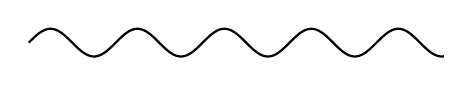
\begin{tikzpicture}
    \begin{axis}[
      x=5pt,
      y=5pt,
      clip bounding box=upper bound,
      hide axis,
      thick,
      ]
      \addplot[domain=0:30,samples=300]{sin(x*180/pi)};
    \end{axis}
  \end{tikzpicture}
  \medskip

  Señal discreta: digital
  \smallskip

  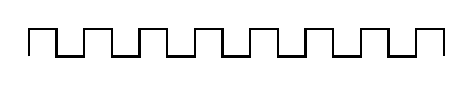
\begin{tikzpicture}
    \begin{axis}[
      x=10pt,
      y=10pt,
      clip bounding box=upper bound,
      hide axis,
      thick
      ]
      \addplot[domain=0:30,samples=300,const plot] coordinates 
        {(0,0) (0,1) (1,0) (2,1) (3,0) (4,1) (5,0) (6,1) (7,0)
          (8, 1)
          (9, 0)
          (10, 1)
          (11, 0)
          (12, 1)
          (13, 0)
          (14, 1)
          (15, 0)
        };
    \end{axis}
  \end{tikzpicture}
  \\
  AM
  &
  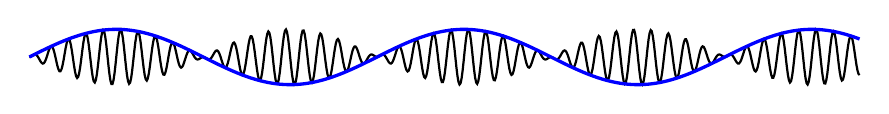
\begin{tikzpicture}
    \begin{axis}[
      x=10pt,
      y=10pt,
      clip bounding box=upper bound,
      hide axis,
      domain=0:30,
      thick
      ]
      \addplot[samples=800]
        {sin(x*180/pi*10) * sin(x*180/pi*0.5)};
      \addplot[blue,very thick,samples=300]
        {sin(x*180/pi*0.5)};
    \end{axis}
  \end{tikzpicture}
  \\
  FM
  &
  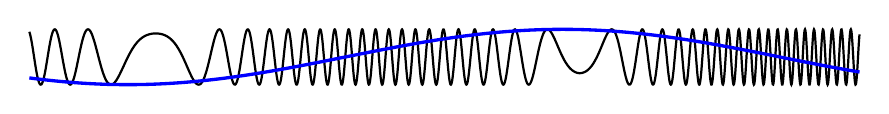
\begin{tikzpicture}
    \begin{axis}[
      x=10pt,
      y=10pt,
      clip bounding box=upper bound,
      hide axis,
      domain=20:50,
      thick
      ]
      \addplot[samples=2500]
        {sin(deg(2*x*sin(deg(x)*0.2))) };
      \addplot[blue,very thick,samples=200]
        {sin(deg(x)*0.2)};
    \end{axis}
  \end{tikzpicture}
\end{longtblr}


\vspace{16pt}


\end{document}

